\chapter{Les Missions réalisées}
\section{Enjeux et cadre des missions effectuées}
Ma première mission était la réalisation d'une application mobile multi-plateforme 
reprennant les fonctionnalités du site web client tout en prenant en compte 
les différences d'expérience utilisateur qu'apporte une interface tactile.\newline

Les outils et technologies utilisées pour cette mission sont les suivantes:

\begin{figure}[!h]
    \centering
    \begin{minipage}[b]{0.4\textwidth}
      
\includegraphics[width=\textwidth]{Images/ionic-logo}
    \end{minipage}
    \hfill
    \begin{minipage}[b]{0.4\textwidth}
      
\includegraphics[width=\textwidth]{Images/ajsthtml5}
    \end{minipage}
  \end{figure}

\begin{itemize}
    \item Ionic + cordova
    \item Git comme outils de versionning de code source
    \item Npm comme gestionnaire de librairie 
    \item Visual Studio Code
    \item GitLab pour l'hebergement du code source et la gestion de projet \newline
\end{itemize} 

La seconde mission était la refonte totale du site web client qui contient aussi l'API pour 
l'application mobile, ce nouveau site nommé web3 doit avoir les mêmes fonctionnalitées que 
la version précédente tout en utilisant la puissance des nouvelles technologies. \newline

\begin{itemize}
    \item client-side: version Progressive Web App de l'application mobile 
    \item server-side: Asp.net Core 
    \item persistance: base de donnée NexusDB
    \item Git comme outils de versionning de code source 
    \item GitLab pour l'hebergement du code source et la gestion de projet 
    \item Visual Studio Code \newline
\end{itemize}



\section{Présentation d'une mission à fort enjeux: le site client}
Le site web client est la facade directement visible de nos clients c'est donc un produit crucial pour
l'entreprise, il m'a été confié la création du nouveau site web, appelé en interne web3 car il s'agit de la troisième
refonte du site.

j'ai eu totale liberté pour le choix des technologies utilisés, le web2 est basé sur un stack vieillissant: asp.net webforms et jquery.
De plus, la qualité du code et sa maintenabilité est extrèmement faible rendant difficile et ce de manière 
exponentielle, l'ajout de fonctionnalitées et la correction de bugs. 

Pour les choix techniques j'ai choisis de rester sur l'utilisation du langage C\# pour deux raisons, tout d'abord 
je maitrise ce langage depuis de nombreuses années et ensuite c'est le langage utilisé dans la réalisation de tout les 
autres logiciels au sein de l'entreprise ce qui assure une certaine homogeneité et enfin cela me permet 
aussi de reprendre le code de l'ancien site client plus facilement. \newline

L'architecture du web2 était completement incorrecte, utilisant le C\# comme langage purement procédural plutot que 
comme langage objet, aucune des bonnes pratiques ne sont respecté ce qui rend le code hautement dupliqué 
et difficile à maintenir, de plus aucun test unitaires n'etait mis en place rendant difficile la non-regressions.

La première étape fut d'analyser ce qui appartenait purement à la partie métier et l'isoler des composants 
techniques relatif à l'application et à la persistance des données: \newline

\begin{figure}[h]
	\centering
	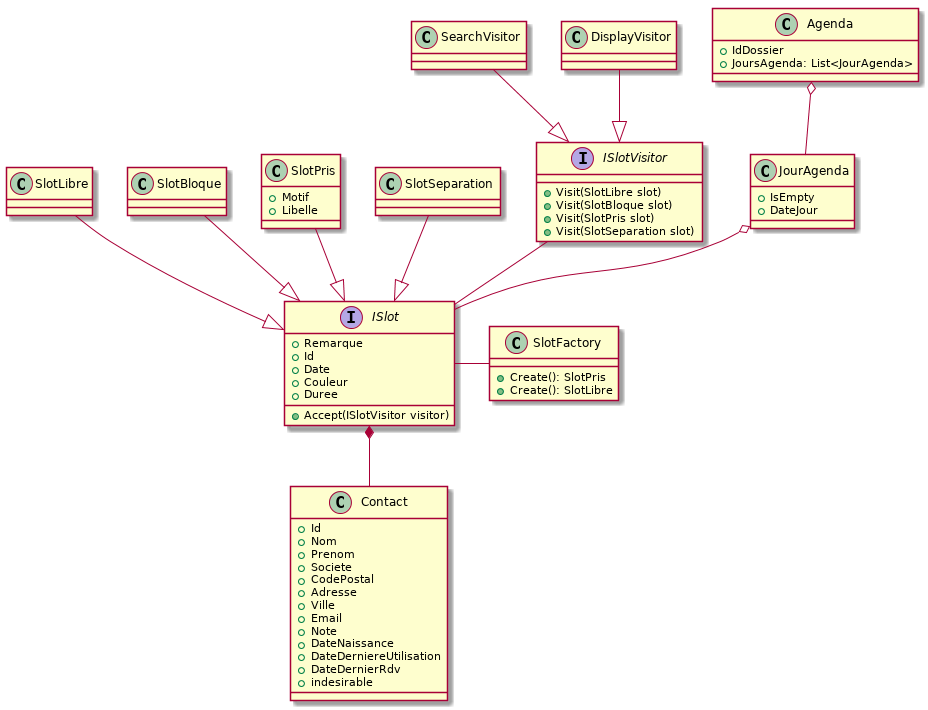
\includegraphics[width=1\linewidth]{Images/slotmodelold}
	\caption{classes métier pour l'agenda}
	\label{fig:domainagenda}
\end{figure}

\begin{figure}[h]
	\centering
	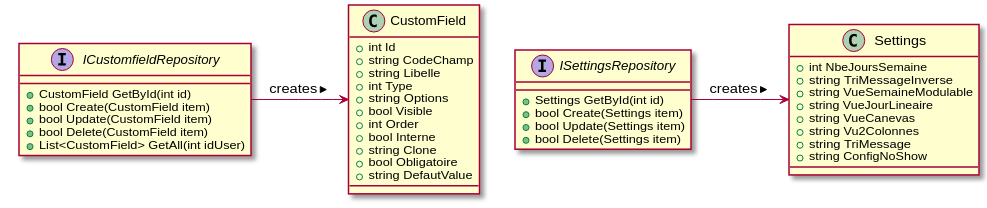
\includegraphics[width=1\linewidth]{Images/otherpersistence}
	\caption{reste des classes métier}
	\label{fig:otherrepo}
\end{figure}

\begin{figure}[h]
	\centering
	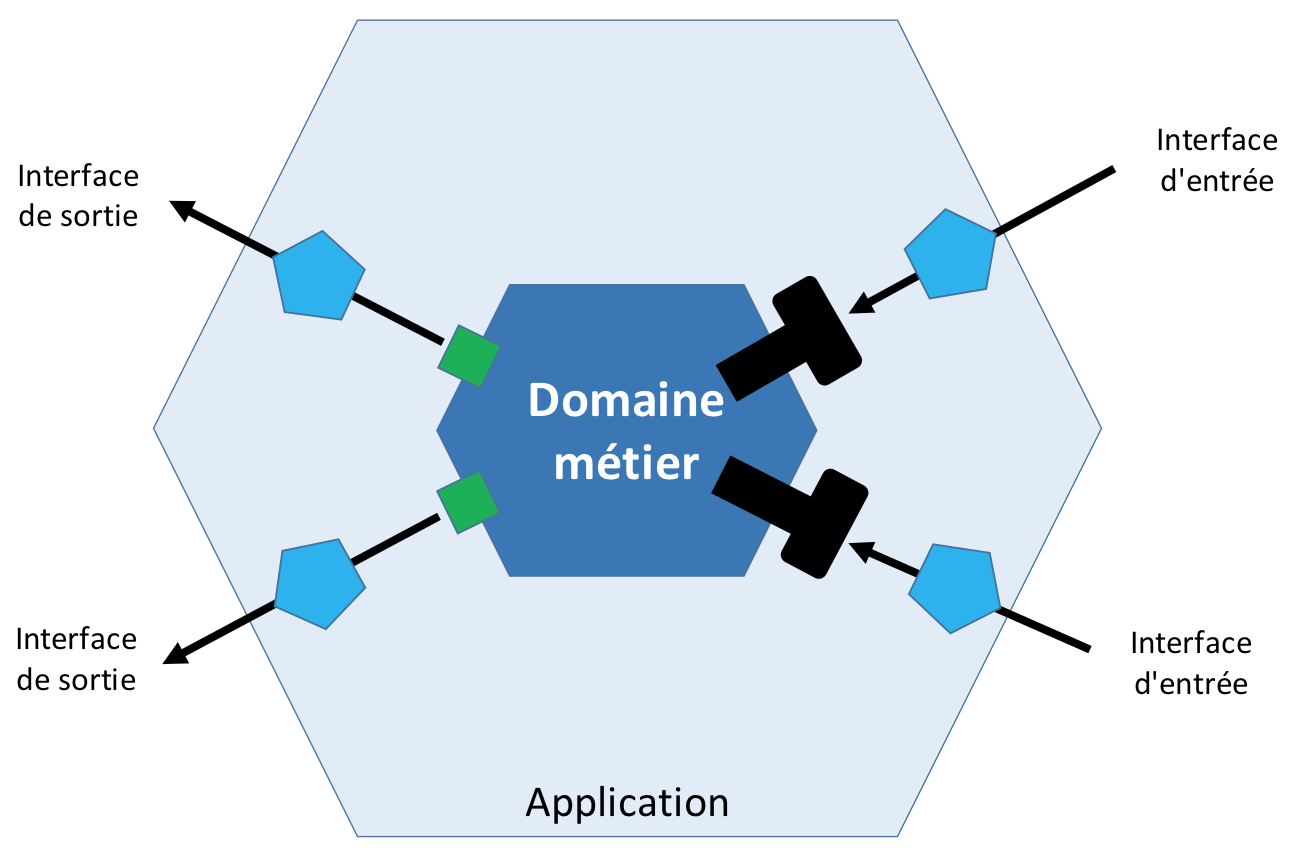
\includegraphics[width=0.8\linewidth]{Images/hexarch}
	\caption{Architecture Hexagonale}
	\label{fig:archhexa}
\end{figure}


\newpage

\section{Bilan et recul sur les missions}
Sur le plan professionnel cette année a été très enrichissante, j'ai pu renforcer mes compétences dans 
les framework Angular, Ionic et .NET que j'avais commencé à acquérir lors de mon année de licence 
professionnelle, sur le projet de site web j'ai pu appliquer pleinement mes compétences 
dans l'architecture des logiciels avec la mise en place de méthodes de développement et 
de gestion de projet agile dans un premier temp puis avec l'application des bonnes pratiques 
de développement pour les langages orientés object avec l'utilisation correcte de design pattern
et le respect des règles de base pour la création de logiciels maintenable, performant et fiables.
\newline

D'un point de vu personnel j'ai appris beaucoup de choses sur la gestion d'agenda et les centres d'accueil téléphonique notamment
en terme de contraintes techniques qui sont imposées par des clients réticent au changement 
ainsi que les enjeux technologiques de ce cœur de métier qui doit se faire peau neuve 
pour rester compétitif.

Le marché de la prise de rendez-vous évolue et se tourne de plus en plus vers le 
web et le mobile, j'ai apporté à Eurice les compétences pour la réalisation d'application 
Mobile sur les plateformes Android et iOS\newline
